% not fixed

\chapter{METODOLOGI}
\label{chap:metodologi}

% Ubah bagian-bagian berikut dengan isi dari desain dan implementasi

Pelaksanaan tugas akhir ini dilaksanakan sesuai dengan metodologi yang telah dibuat, juga dengan implementasinya. Metodologi merupakan konsep dari pembuatan dan perancangan infrastruktur dan kemudian diwujudkan dalam bentuk blok-blok alur diagram yang harus dikerjakan. Pada bagian implementasi merupakan pelaksanaan teknis untuk setiap blok pada metodologi.

\begin{figure}[H]
    \centering
    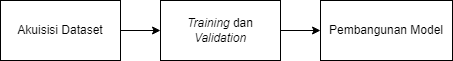
\includegraphics[scale=0.9]{gambar/metodologi_umum.png}
    \caption{Blok Diagram Metodologi}
    \label{fig:desainsistem}
\end{figure}

\section{Peralatan}
\label{sec:peralatan}
Peralatan yang digunakan pada pelaksanaan tugas akhir ini yaitu perangkat laptop dan \textit{smartphone.} Laptop, digunakan pada keseluruhan implementasi metodologi. Adapun spesifikasi laptop yang digunakan pada pelaksanaan tugas akhir ini adalah laptop dengan spesifikasi seperti pada Tabel \ref{tb:spesifikasilaptop}.\par

\begin{table}[H]
    \begin{center}
    \caption{Spesifikasi Perangkat Laptop yang Digunakan}
    \label{tb:spesifikasilaptop}
    \begin{tabular}{|l|l|}
        \hline
        \textit{\textbf{Processor}}        & \begin{tabular}[c]{@{}l@{}}Intel Core i5-8300H \\ CPU @ 2.3 GHz (8 CPUs)\end{tabular} \\ \hline
        \textit{\textbf{Storage}}          & \begin{tabular}[c]{@{}l@{}}HDD 1 TB Storage\\ SSD 256 GB Storage\end{tabular}         \\ \hline
        \textit{\textbf{RAM}}              & \begin{tabular}[c]{@{}l@{}}16 GB SODIMM DDR4 \\ 2667 MHz Dual Channel\end{tabular}    \\ \hline
        \textit{\textbf{Graphic Card}}     & \begin{tabular}[c]{@{}l@{}}NVIDIA GeForce GTX 1050 Ti \\ 4 GB GDDR5\end{tabular}      \\ \hline
        \textit{\textbf{Operating System}} & \begin{tabular}[c]{@{}l@{}}Windows 10 Home \\ Single Language 64-bit\end{tabular}     \\ \hline
    \end{tabular}
    \end{center}
\end{table}

Selain perangkat laptop, perangkat \textit{smartphone} juga digunakan khususnya pada proses pengambilan citra dataset serta citra untuk pengujian. Adapun spesifikasi \textit{smartphone} yang digunakan pada pelaksanaan tugas akhir ini yaitu seperti pada Tabel \ref*{tb:spesifikasismartphone}. \par

\begin{table}[H]
    \centering
    \caption{Spesifikasi Perangkat \textit{Smartphone} yang Digunakan}
    \label{tb:spesifikasismartphone}
    \begin{tabular}{|l|l|}
    \hline
    \textbf{Jenis Smartphone}   & Samsung Galaxy A7 2018                                                                                                                                          \\ \hline
    \textbf{Spesifikasi Kamera} & \begin{tabular}[c]{@{}l@{}}24 MP, f/1.7, 27mm (wide), 1/2.8", 0.9µm, PDAF \\ 8 MP, f/2.4, 18mm (ultrawide), 1/4.0", 1.12µm \\ 5 MP, f/2.2, (depth)\end{tabular} \\ \hline
    \end{tabular}
    \end{table}

\section{Metodologi}
\label{sec:desainsistem}

Tugas akhir ini merupakan penelitian dalam bidang visi komputer yang bertujuan untuk mendeteksi huruf balok tulisan tangan pada media papan tulis menggunakan metode \textit{you only look once} (YOLO). Secara umum alur blok diagram metodologi yaitu seperti yang telah dibuat pada Gambar \ref*{fig:desainsistem}. Perancangan model menggunakan metode YOLO, lebih spesifik yaitu YOLOv5. \par

Berdasarkan Gambar \ref*{fig:desainsistem}, langkah awal yang harus dilakukan yaitu proses akuisisi dataset, yaitu dengan mengumpulkan data tulisan tangan huruf balok pada media papan tulis dan setelahnya juga dilakukan pre-proses tertentu yang akan dijelaskan pada sub akuisisi data. Proses selanjutnya yaitu dengan melakukan konfigurasi-konfigurasi \textit{hyperparameter} pada model sebelum dilakukan training, dan ketika sudah dilakukan proses training maka hasil model yang telah dibuat tersebut dievaluasi dengan \textit{evaluation metrics} yang telah ditentukan sebelumnya. Setelah model selesai dievaluasi dan hasilnya sudah mencapai \textit{threshold} tertentu, maka proses selanjutnya yaitu pembangunan model untuk konversi gambar menjadi teks. \par

% Per blok diagram dijelaskan dan dibuatkan section masing-masing

\section{Akuisisi Dataset}
\label{sec:akuisisidataset}

Dalam pelaksanaan proses akuisisi dataset, terdapat beberapa bagian proses yang harus dilakukan yang dapat dilihat pada blok diagram berikut.

\begin{figure}[H]
    \centering
    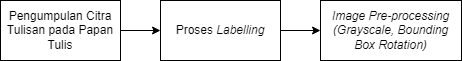
\includegraphics[scale=0.9]{gambar/metodologi_akuisisi_data.png}
    \caption{Alur Akuisisi Dataset}
    \label{fig:alurakuisisidataset}
\end{figure}

\subsection{Pengumpulan Citra Tulisan pada Papan Tulis}
\label{subsec:pengumpulancitra}

Proses pengumpulan citra huruf balok tulisan tangan pada papan tulis dimulai dengan menentukan jumlah kelas dataset yang akan digunakan. Adapun kelas dataset nantinya akan terdiri dari huruf, angka, dan simbol. Pada huruf alfabet, terdapat 26 huruf dari A sampai Z, namun hanya 19 kelas yang akan digunakan (kecuali huruf C, F, O, Q, X, Y, Z) yang artinya pada proses akuisisi dataset ini nantinya akan terdapat 19 kelas yang mewakili huruf tersebut. Sedangkan pada angka terdapat 10 angka dari 0 sampai 9, yang artinya akan terdapat 10 kelas yang mewakili masing-masing angka tersebut. Sehingga total kelas yang digunakan yaitu 19 kelas angka, 10 kelas angka, dan 2 kelas simbol ('=' dan '*'). Setelah jumlah kelas ditentukan, proses selanjutnya yaitu membuat huruf balok tulisan tangan pada media papan tulis kemudian melakukan pengambilan citra dari huruf balok tulisan tangan yang telah dituliskan pada media papan tulis tersebut. Proses tersebut diulang sebanyak beberapa kali pada tiap kelas yang sama dan diulang kembali sesuai jumlah kelas yang tersedia. \par

\subsection{Proses Pelabelan Dataset}
\label{subsec:proseslabelling}

Proses pelabelan yaitu merupakan proses pemberian label dengan memberikan \textit{bounding box} pada objek dan nama kelas pada objek tersebut. Tujuan dari proses pelabelan ini yaitu untuk mendapatkan \textit{ground-truth bounding box}. Proses pelabelan dilakukan dengan menggunakan bantuan \textit{tool} yaitu Roboflow. Sebelum proses pelabelan dilakukan, citra yang telah dikumpulkan sebelumnya diupload pada \textit{workspace} Roboflow. Proses pelabelan dataset secara sederhana seperti terlihat pada Gambar \ref*{fig:ilustrasipelabelan}. Setelah seluruh citra yang termasuk dalam kelas objek telah diberi anotasi \textit{bounding box}, seluruh citra selanjutnya dibagi menjadi \textit{training set}, \textit{validation set}, dan juga \textit{testing set} (opsional). \par
% Adapun pembagian \textit{training testing sets} menggunakan komposisi 80\% \textit{training sets} dan 20\% \textit{testing sets}. \par

\begin{figure}[H]
    \begin{subfigure}{.5\textwidth}
      \centering
      \captionsetup{width=.8\linewidth}
      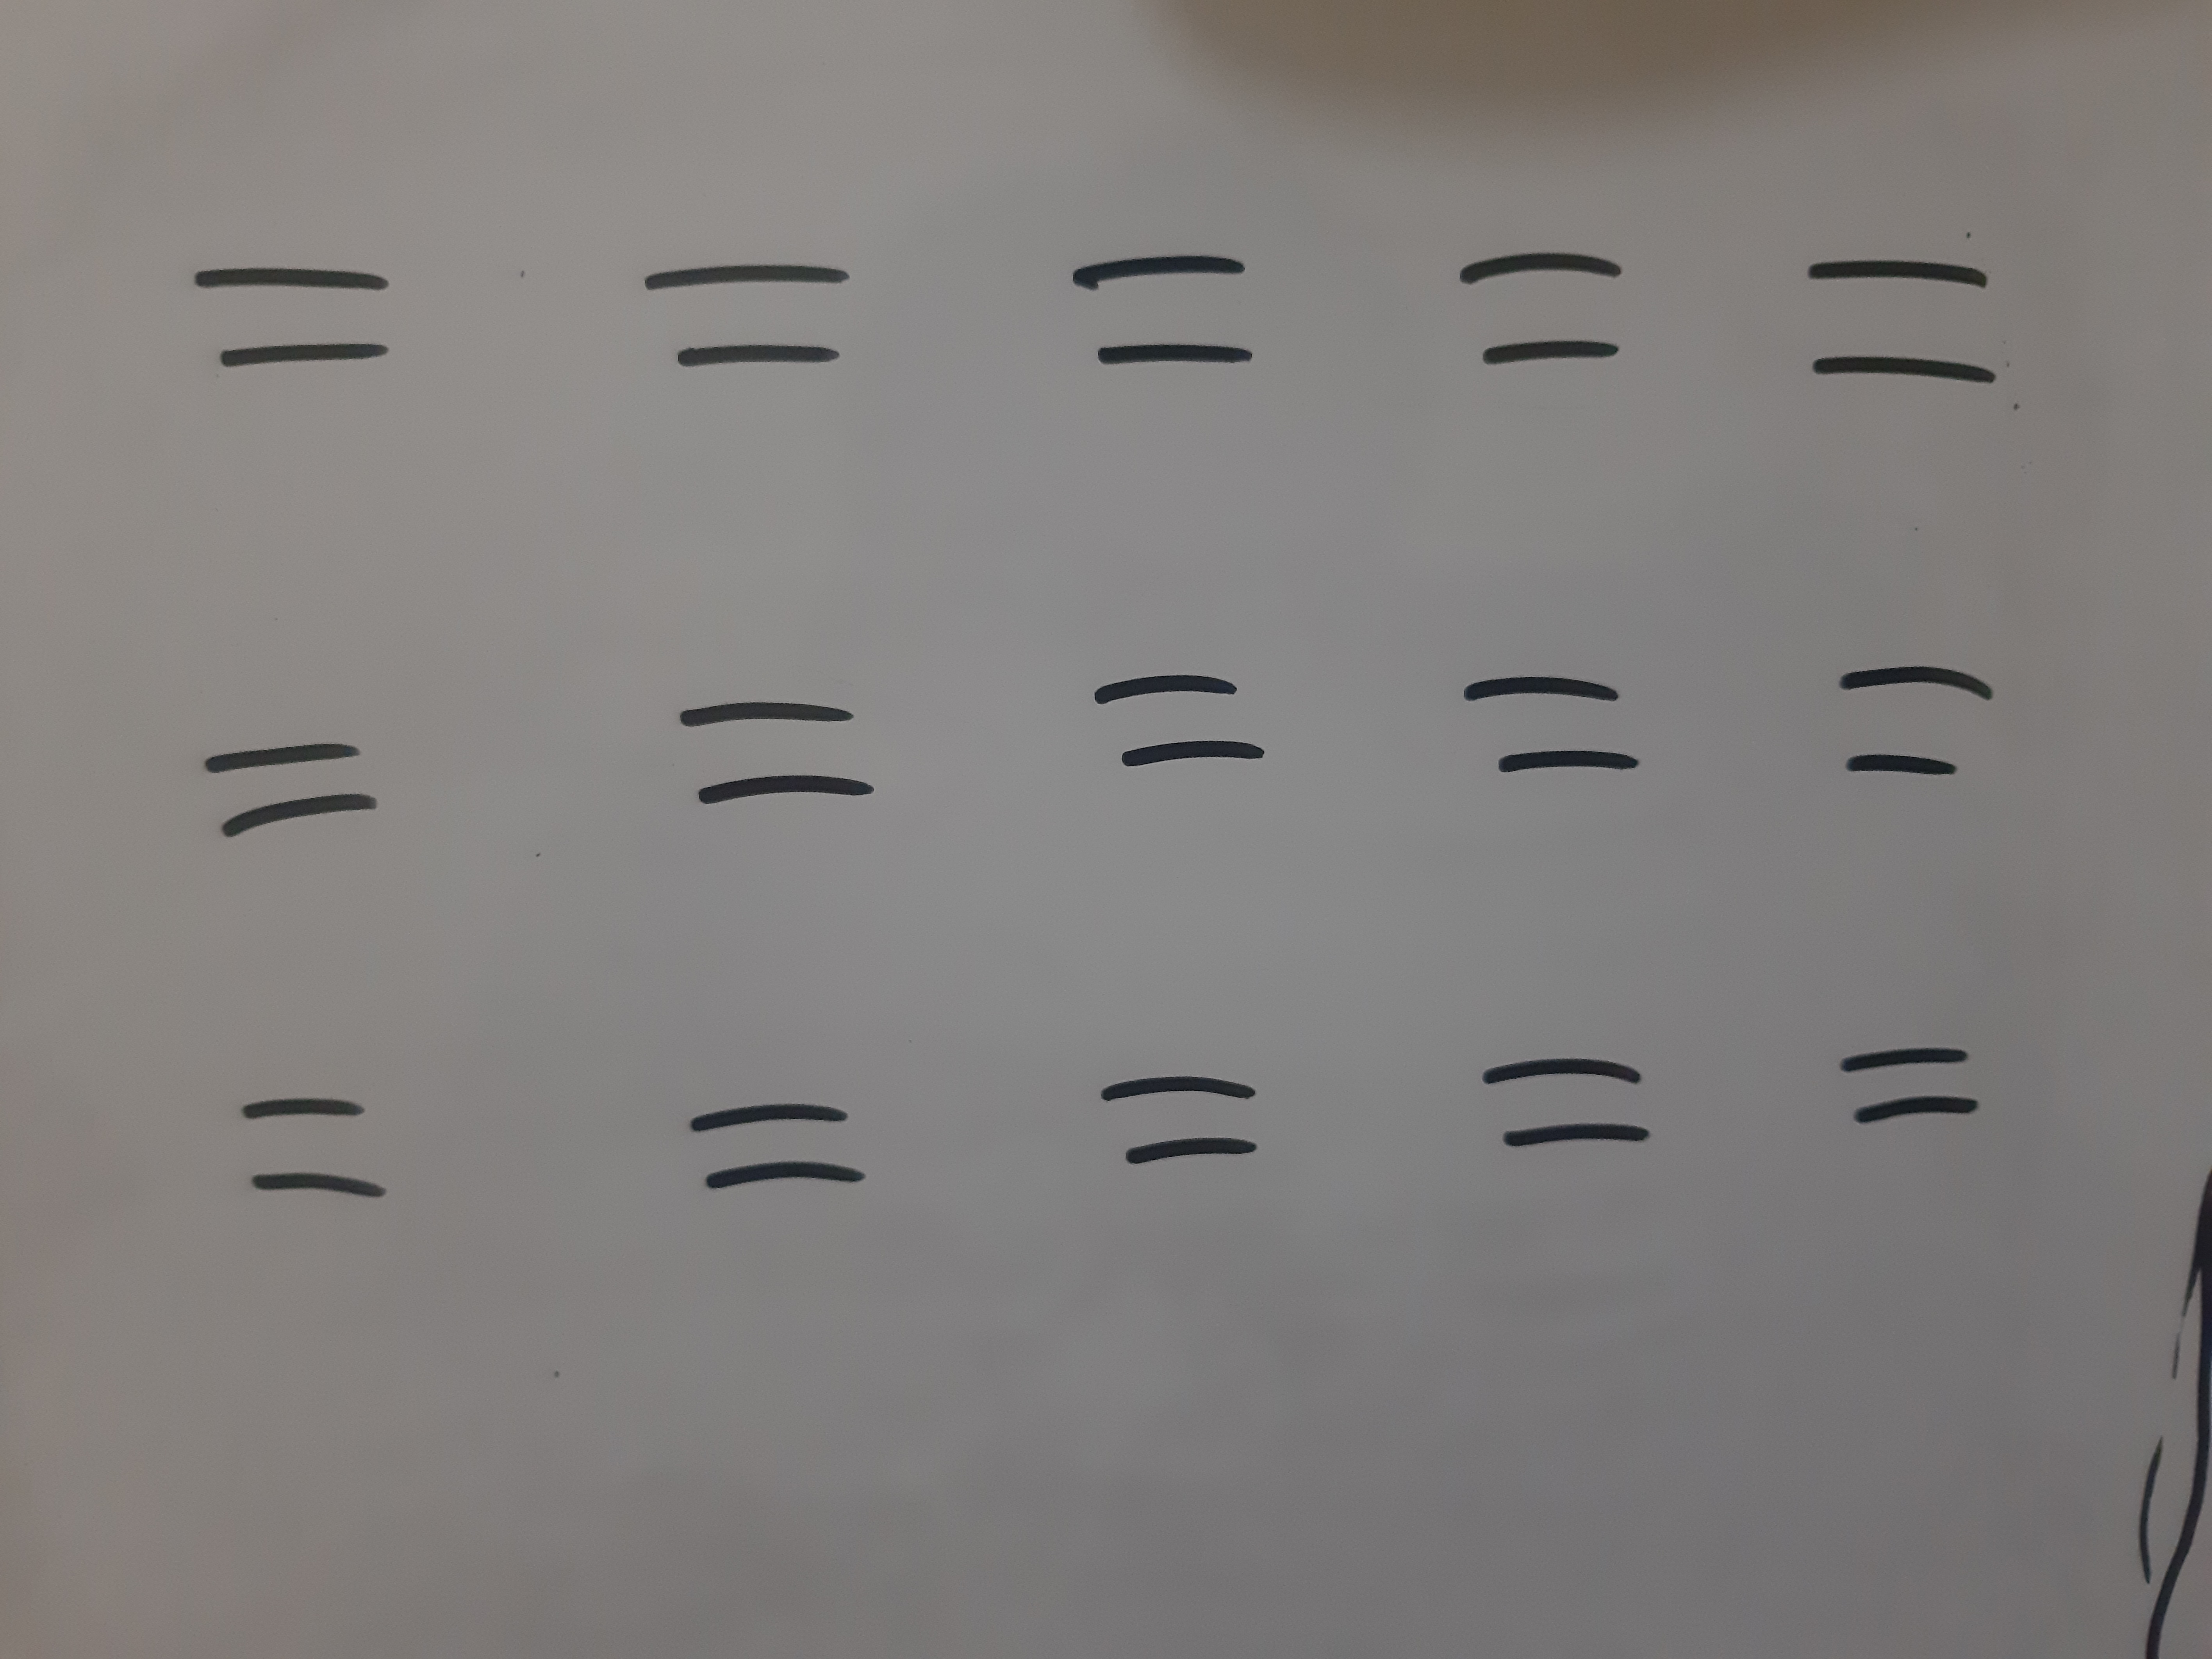
\includegraphics[width=.85\linewidth]{gambar/label_before.jpg}
      \caption{Sebelum Proses Pelabelan}
      \label{fig:labelbefore}
    \end{subfigure}%
    \begin{subfigure}{.5\textwidth}
      \centering
      \captionsetup{width=.8\linewidth}
      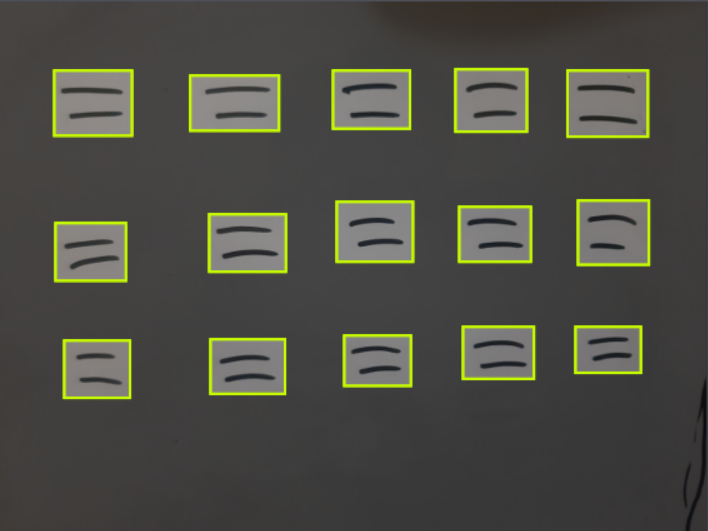
\includegraphics[width=.85\linewidth]{gambar/label_after.png}
      \caption{Setelah Proses Pelabelan}
      \label{fig:labelafter}
    \end{subfigure}
    \caption{Ilustrasi Proses Pelabelan Dataset}
    \label{fig:ilustrasipelabelan}
  \end{figure}

\subsection{\textit{Image Pre-Processing}}
\label{subsec:imagepreprocess}
Pada tahap \textit{pre-process}, citra yang telah diberi label selanjutnya dilakukan \textit{pre-process} tertentu. Tahapan \textit{pre-process} bertujuan untuk mengurangi waktu \textit{training} dan meningkatkan performa. Tahapan \textit{pre-process,} secara umum terbagi menjadi 2 tingkatan yaitu \textit{image level pre-process} dan \textit{bounding box level pre-process} atau augmentasi. \textit{Image level pre-process} yaitu pemrosesan pada tingkat citra, artinya proses yang dilakukan pada tingkatan ini berlaku untuk seluruh dataset yang dimiliki, sedangkan pada \textit{bounding box level pre-process} bertujuan untuk memperbanyak dataset dengan memberikan transformasi tertentu kemudian menduplikat sebanyak jumlah tertentu dan data yang diduplikat hanya yang berada pada \textit{training set}. Pada tahapan \textit{image pre-processing} ini dilakukan berbagai jenis \textit{image level pre-process} yaitu sebagai berikut: \par
\begin{enumerate}[nolistsep]
    \item \textit{\textbf{Resize.} Resize} yaitu proses perubahan dimensi dari suatu citra pada dataset. Proses ini bertujuan untuk memperkecil atau memperbesar ukuran file sehingga ketika diproses dapat memberikan hasil yang lebih baik. 
    % Adapun pada tugas akhir ini, proses \textit{resize} yang digunakan yaitu \textit{strecth to} 416x416. Penggunaan \textit{strecth to} 416x416 dilakukan agar ukuran citra dapat menjadi kecil, sehingga mempermudah dan mempercepat proses \textit{training} mengingat jumlah kelas dan jumlah data yang cukup banyak.
    \begin{figure}[H]
        \centering
        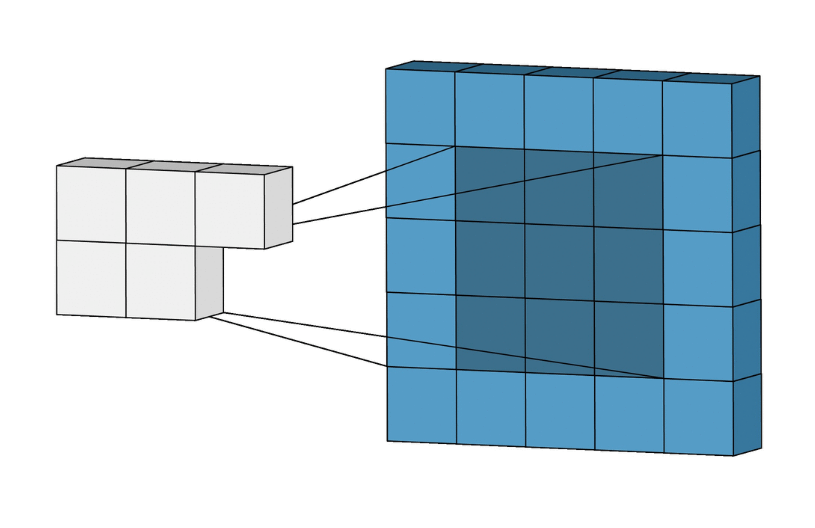
\includegraphics[scale=0.5]{gambar/imageresize.png}
        \caption{Ilustrasi \textit{Image Resize} dalam Skala Piksel}
        \label{fig:imageresize}
    \end{figure}

    \item \textit{\textbf{Auto Orient.} Auto Orient} menghapus suatu citra dari EXIF datanya sehingga citra yang ditampilkan sesuai dengan citra yang ada pada penyimpanan. Data EXIF umumnya menentukan orientasi dari suatu citra. Ketika suatu citra diambil, citra tersebut berisi \textit{metadata} yang menentukan orientasi yang harus ditampilkan relatif terhadap bagaimana piksel diatur pada penyimpanan.
    \item \textit{\textbf{Filter Null.}} Dalam mempersiapkan suatu dataset untuk sebuah model \textit{deep learning,} mengelola anotasi data merupakan suatu hal yang cukup menantang, bahkan dengan asumsi citra \textit{train} representatif ketika dilakukan \textit{inference.} Salah satu tantangannya yaitu menentukan apakah suatu citra memiliki anotasi atau tidak (baik itu disengaja atau tidak sengaja). \textit{Missing annotation} terjadi ketika suatu cita memiliki objek yang tidak dianotasi dengan baik, hal ini menjadi permasalahan mengingat suatu model akan di-\textit{train} berdasarkan \textit{"false negatives"} dari objek. \textit{Null Annotation} terjadi ketika suatu citra tidak memiliki objek sehingga tidak diperlukannya suatu anotasi. Dengan adanya \textit{Filter Null} ini maka diharapkan model yang dibuat dapat lebih akurat. Contoh citra yang tidak memiliki objek kelas apapun yaitu seperti Gambar \ref*{fig:nullimage} berikut.
    \begin{figure}[H]
        \centering
        
\includegraphics[scale=0.04]{gambar/null_image.jpg}
        \caption{Contoh Citra yang Tidak Memiliki Objek Kelas}
        \label{fig:nullimage}
    \end{figure}
    \item \textit{\textbf{Contrast.} Contrast} merupakan perbedaan kondisi yang dapat diamati. Dalam konteks citra, berarti perbedaan kondisi ketika menangkap suatu objek yang jelas. Lebih jauh, \textit{contrast} sebenarnya tidak menggunakan konsep memberikan \textit{blanket ffilter} untuk meningkatkan/mengurangi piksel, namun lebih kepada piksel dalam suatu citra disesuaikan secara relatif. Salah satu konsep fundamental dalam visi komputer yaitu \textit{"edge detection".} Ketika menggunakan \textit{contrast} dalam \textit{image pre-processing,} tepian-tepian menjadi lebih terlihat perbedannya.
    \item \textit{\textbf{Grayscale.}} Pada proses \textit{grayscale}, citra dikonversi dengan \textit{channel rgb} menjadi suatu citra dengan hanya sebuah \textit{channel grayscale,} sehingga dapat menghemat memori. Pada proses \textit{grayscale,} citra pada dataset tugas akhir ini dikonversi menjadi warna abu dengan tujuan untuk memperkecil variasi warna spidol pada media papan tulis sehingga model yang dibuat berfokus hanya pada pola tulisan tangan pada papan tulis saja dan tidak terfokus ke warna yang digunakan untuk menulis pada papan tulisnya.
    % \item \textit{\textbf{Filter Null.}}
    % \item \textit{\textbf{Blur.}}
    % \item \textit{\textbf{Noise.}}
    % \item \textit{\textbf{Bounding Box Rotation.}}
\end{enumerate}

% Terakhir, dilakukan proses \textit{bounding box rotation}, yaitu melakukan rotasi pada skala \textit{bounding box}. Tujuan dari proses \textit{bounding box rotation} yaitu untuk menambah variasi sehingga model yang tercipta lebih akurat ketika pengambilan citra tidak diambil tepat didepan objek. 
% Adapun konfigurasi dari \textit{bounding box rotation} yaitu antara -15\textdegree\space dan +15\textdegree. \par

\section{\textit{Training} dan \textit{Validation}}
\label{sec:trainvaldata}

\textit{Training data} dilakukan setelah proses pengumpulan citra, proses pelabelan, dan pre-proses gambar selesai dilaksanakan. Dalam proses \textit{training}, dibutuhkan konfigurasi \textit{hyperparameter} tertentu seperti jumlah epochs, \textit{batch size}, dan jenis \textit{pretrained weight} yang akan digunakan. Pada tugas akhir ini, versi YOLO yang digunakan yaitu YOLOv5. Sebelum proses \textit{training} dilakukan, perlu ditentukan jenis \textit{pretrained weights} yang akan digunakan. \par

YOLOv5 memiliki beberapa varian \textit{pretrained weights} model yang tersedia yaitu YOLOv5n, YOLOv5s, YOLOv5m, YOLOv5l, dan YOLOv5x. Secara umum perbedaan antar \textit{pretrained weight} yang ada yaitu pada \textit{pretrained weight} model yang lebih besar seperti YOLOv5x dapat menghasilkan hasil yang lebih baik ditinjau hampir dari seluruh aspek yang ada, namun model tersebut akan memiliki lebih banyak parameter sehingga membutuhkan lebih banyak memori CUDA untuk melakukan \textit{train} sehingga membutuhkan waktu pemrosesan yang relatif lebih lama dibandingkan versi lebih sederhananya yaitu YOLOv5s. Perbedaan performa pada varian YOLOv5 dapat dilihat pada Gambar \ref*{fig:yolov5comparison} berikut dengan catatan seluruh data \textit{checkpoints} di-\textit{train} dengan 300 epochs dan pengaturan \textit{default}. Secara spesifik, perbandingan varian YOLOv5 dapat dilihat pada Gambar \ref*{fig:yolov5comparison}. \par

\begin{figure}[H]
    \centering
    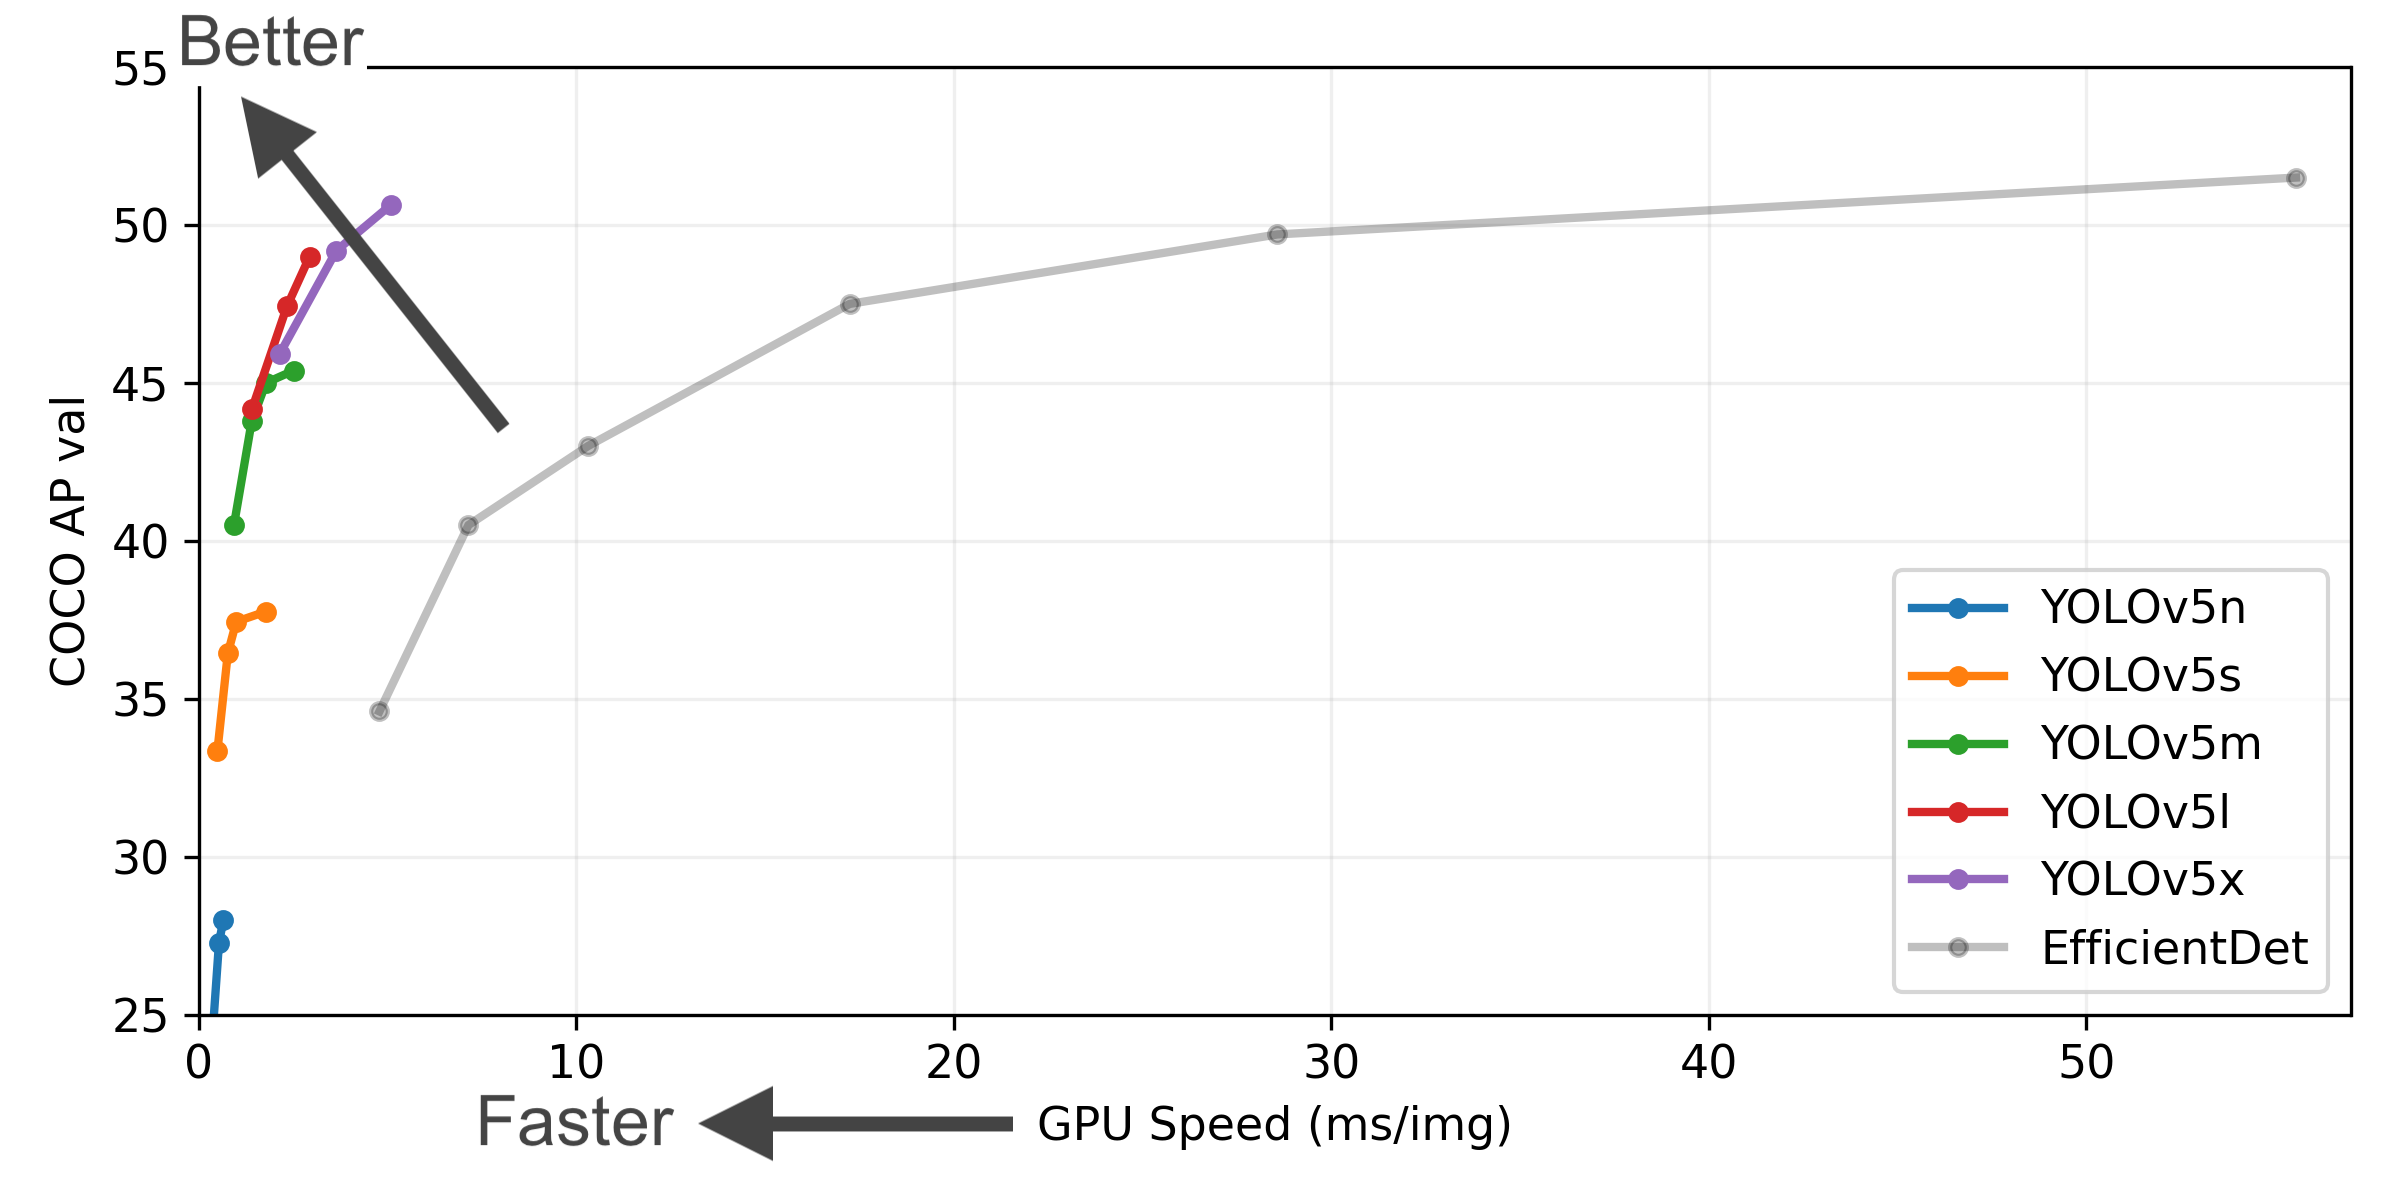
\includegraphics[scale=0.75]{gambar/yolov5comparison.png}
    \caption{Perbandingan Performa dan Akurasi Antar Varian YOLOv5 \citep*{ultralyticsyolo}}
    \label{fig:yolov5comparison}
\end{figure}
% Adapun konfigurasi layer YOLOv5 secara lebih lengkap telah dibahas pada tinjauan pustaka ttg yolov5 

Sebelum melakukan proses \textit{train} menggunakan YOLO (YOLOv5s), perlu dilakukan konfigurasi \textit{hyperparameter} terlebih dahulu. Adapun konfigurasi \textit{hyperparameter} yang akan dilakukan pada YOLOv5s untuk dataset yang akan di-\textit{train} yaitu: \par

\begin{enumerate}[nolistsep]
    \item \textbf{Epochs.} Epochs adalah \textit{hyperparameter} yang berfungsi untuk menentukan jumlah pengulangan atau berapa kali suatu algoritma \textit{learning} akan melakukan proses \textit{learning} suatu \textit{dataset training}. Secara sederhana, semakin besar jumlah epochs maka model yang dihasilkan memiliki tingkat akurasi yang lebih tinggi namun waktu yang dibutuhkan untuk melakukan \textit{learning} akan semakin lambat. 
    \item \textit{\textbf{Batch-Size.} Batch-size} adalah \textit{hyperparameter} yang berfungsi untuk mengontrol jumlah sampel training untuk dikerjakan sebelum parameter internal model diperbarui. 
    \item \textit{\textbf{Image Size.}} \textit{Image size} adalah dimensi ukuran citra yang diterapkan pada \textit{dataset}. Secara sederhana, semakin kecil dimensi ukurang dari suatu citra maka akan semakin singkat waktu yang dibutuhkan untuk melakukan proses \textit{training}.
    \item \textit{\textbf{Learning Rate.} Learning rate \textnormal{adalah} hyperparameter} yang mengontrol seberapa besar perubahan suatu model dalam menanggapi estimasi kesalahan pada tiap kali \textit{weight model} diperbarui. Pemilihan nilai \textit{learning rate} yang tepat diperlukan karena ketika nilai \textit{learning rate} terlalu kecil maka dapat mengakibatkan proses \textit{train} yang lama, sedangkan jika nilai \textit{learning rate} terlalu besar maka dapat mengakibatkan proses \textit{learning} yang kurang optimal dan terlalu cepat atau proses \textit{train} yang tidak stabil.
    \item \textit{\textbf{Optimizer.} Optimizer} merupakan algoritma atau metode yang digunakan untuk meminimisasi eror \textit{(loss function)} atau untuk memaksimalkan efisiensi dari produksi. \textit{Optimizer} merupakan fungsi matematis yang bergantung pada parameter model yang dapat dipelajari seperti \textit{weight \textnormal{dan} biases. Optimizer} sangat membantu untuk mengetahui bagaimana cara mengubah \textit{weights} ataupun \textit{learning rate} dari suatu \textit{neural network} untuk mengurangi nilai \textit{loss} \citep*{optimizerdl}. Jenis \textit{Optimizer} diantaranya yaitu: Adam, \textit{Gradient Descent, \textnormal{dan} Stochastic Gradient Descent (SGD)} \citep*{dlguideoptimizer}. 
\end{enumerate}

Setelah dilakukan proses \textit{training,} maka proses yang dilakukan selanjutnya yaitu proses \textit{validation. \textnormal{Proses} validation} dilakukan untuk mengetahui apakah suatu model yang telah dibuat sebelumnya telah mencapai suatu \textit{threshold} yang telah ditentukan sebelumnya (mencapai nilai akurasi tertentu) atau tidak. Pada proses ini, model tersebut nantinya akan menganalisa menggunakan subset dataset \textit{validation set.} Proses validasi dapat membantu menemukan parameter dan \textit{hyperparameter} yang cocok untuk digunakan pada proses \textit{training} berikutnya serta mencegah terjadinya \textit{overfitting \textnormal{atau} underfitting.} Dalam proses \textit{validation} terdapat alat untuk membantu proses validasi yaitu \textit{evaluation metrics. Evaluation metrics,} merupakan matriks yang biasa digunakan dalam \textit{machine learning \textnormal{atau} deep learning} untuk mengukur kualitas model secara statistika.

\section{Pembuatan Algoritma Konversi Gambar menjadi Teks}
\label{sec:pembuatanmodel}

Setelah dilakukan proses \textit{validation} dan model yang dibuat telah memiliki nilai akurasi yang tinggi (sesuai dengan \textit{threshold} yang telah ditentukan), maka hasil dari proses \textit{training} tersebut secara \textit{default} dapat diakses pada  direktori 'runs/train/..'. Pada direktori tersebut didapatkan \textit{checkpoint} hasil model beserta dengan grafik atau detail data hasil pada tiap proses pengulangan. Tahapan selanjutnya yaitu tahapan pembuatan algoritma konversi gambar menjadi teks.\par

Proses penyusunan teks dimulai dari menentukan koordinat seluruh \textit{bounding box} yang tersedia. Setelah koordinat \textit{bounding box} didapat, seluruh \textit{bounding box} yang terbaca dikelompokan berdasarkan kedekatan antara \textit{bounding box} pertama dengan \textit{bounding box} selanjutnya, jika jarak antaranya memenuhi \textit{threshold} tertentu maka akan dikelompokan menjadi 1, dan jika tidak memenuhi maka akan diletakan pada kelompok berikutnya. Adapun prioritas pengelompokan diatur berdasarkan koordinat Y terlebih dahulu kemudian dilanjutkan dengan koordinat X, hal ini bertujuan agar teks yang ditampilkan berurutan dari baris paling atas lalu bergerak kearah X+ (kanan), dan dilanjut pada baris kedua dan seterusnya. Setelah penyortiran dan pengelompokan \textit{bounding box} berdasarkan koordinat X dan Y telah dilakukan, maka selanjutnya seluruh \textit{bounding box} diambil nama kelasnya dan dimunculkan hasilnya pada citra dengan posisi diatas koordinat XY \textit{bounding box} awal tiap kelompok. Adapun alur proses konversi gambar menjadi teks secara sederhana dapat dilihat pada Gambar \ref*{fig:aluralgoritmakonversi} berikut.\par

\begin{figure}[H]
    \centering
    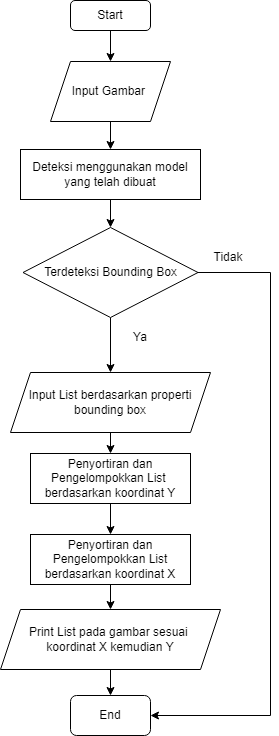
\includegraphics[scale=0.7]{gambar/model_deteksi.png}
    \caption{Alur Algoritma Konversi Gambar Menjadi Teks}
    \label{fig:aluralgoritmakonversi}
\end{figure}
\par

Jika pada suatu citra terdapat persamaan, maka dilakukan proses tambahan untuk mencari nilai hasil dari persamaan tersebut. Adapun proses yang terjadi secara umum yaitu mulanya pada tiap baris dicari kelas '=', apabila terdapat kelas '=' dan kelas simbol lain ('*'), maka baris tersebut merupakan baris persamaan, sedangkan jika hanya terdapat 1 kelas '=' maka baris tersebut merupakan barisan deklarasi variabel dalam persamaan. Setelah seluruh baris terdeteksi, maka proses selanjutnya yaitu pada baris persamaan seluruh persamaannya diisi dengan nilai variabel yang telah dideteksi, sedangkan kelas simbol seperti '*' akan menjadi pengali antar variabelnya. Secara umum, alur tambahan dapat dilihat pada Gambar \ref*{fig:aluralgoritmaperhitungan} berikut. \par

\begin{figure}[H]
    \centering
    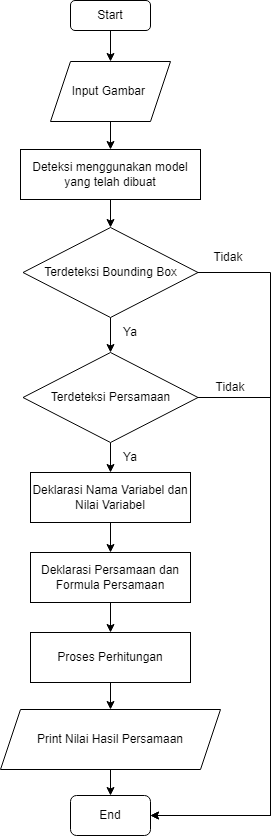
\includegraphics[scale=0.7]{gambar/model_perhitungan.png}
    \caption{Alur Tambahan untuk Algoritma Penyelesaian Persamaan}
    \label{fig:aluralgoritmaperhitungan}
\end{figure}
\par
% alur pembuatan model: start -> input gambar -> deteksi bounding box -> mencari xy bounding box -> pengelompokan berdasarkan y bounding box -> pengelompokan berdasarkan x bounding box -> konversi kelas menjadi bentuk string -> menampilkan label -> selesai
